\chapter{Problem Analysis \& Solution}

Present the solution.

%%-----------------------------------------------------------------------------------------
%%-----------------------------------------------------------------------------------------
\section{Seeing Mesh Difference as a Vector Field}

In our new visualizations, arrows will be used to represent the difference between two triangle meshes. Each arrow will be internally represented by a position and a direction vector. Together, they will form a discrete and bounded vector field. This is a very important abstraction because vector field visualization is a very rich area which finds applications in engineering, molecular modeling and computational fluid dynamics. Therefore, there exist many scientific papers studying this topic, such as \citet{Telea99}, \citet{Garcke00}, \citet{Du04} or \citet{Peng12}.

When visualizing a vector field, it is necessary to use clustering on the vectors to obtain a simplified representation, otherwise the visualization becomes too cluttered (see fig. \ref{fig:meshdiff_unclustered}). Clustering therefore determines to a large extent what the final visualization will look like.

\begin{figure}[h]
\centering
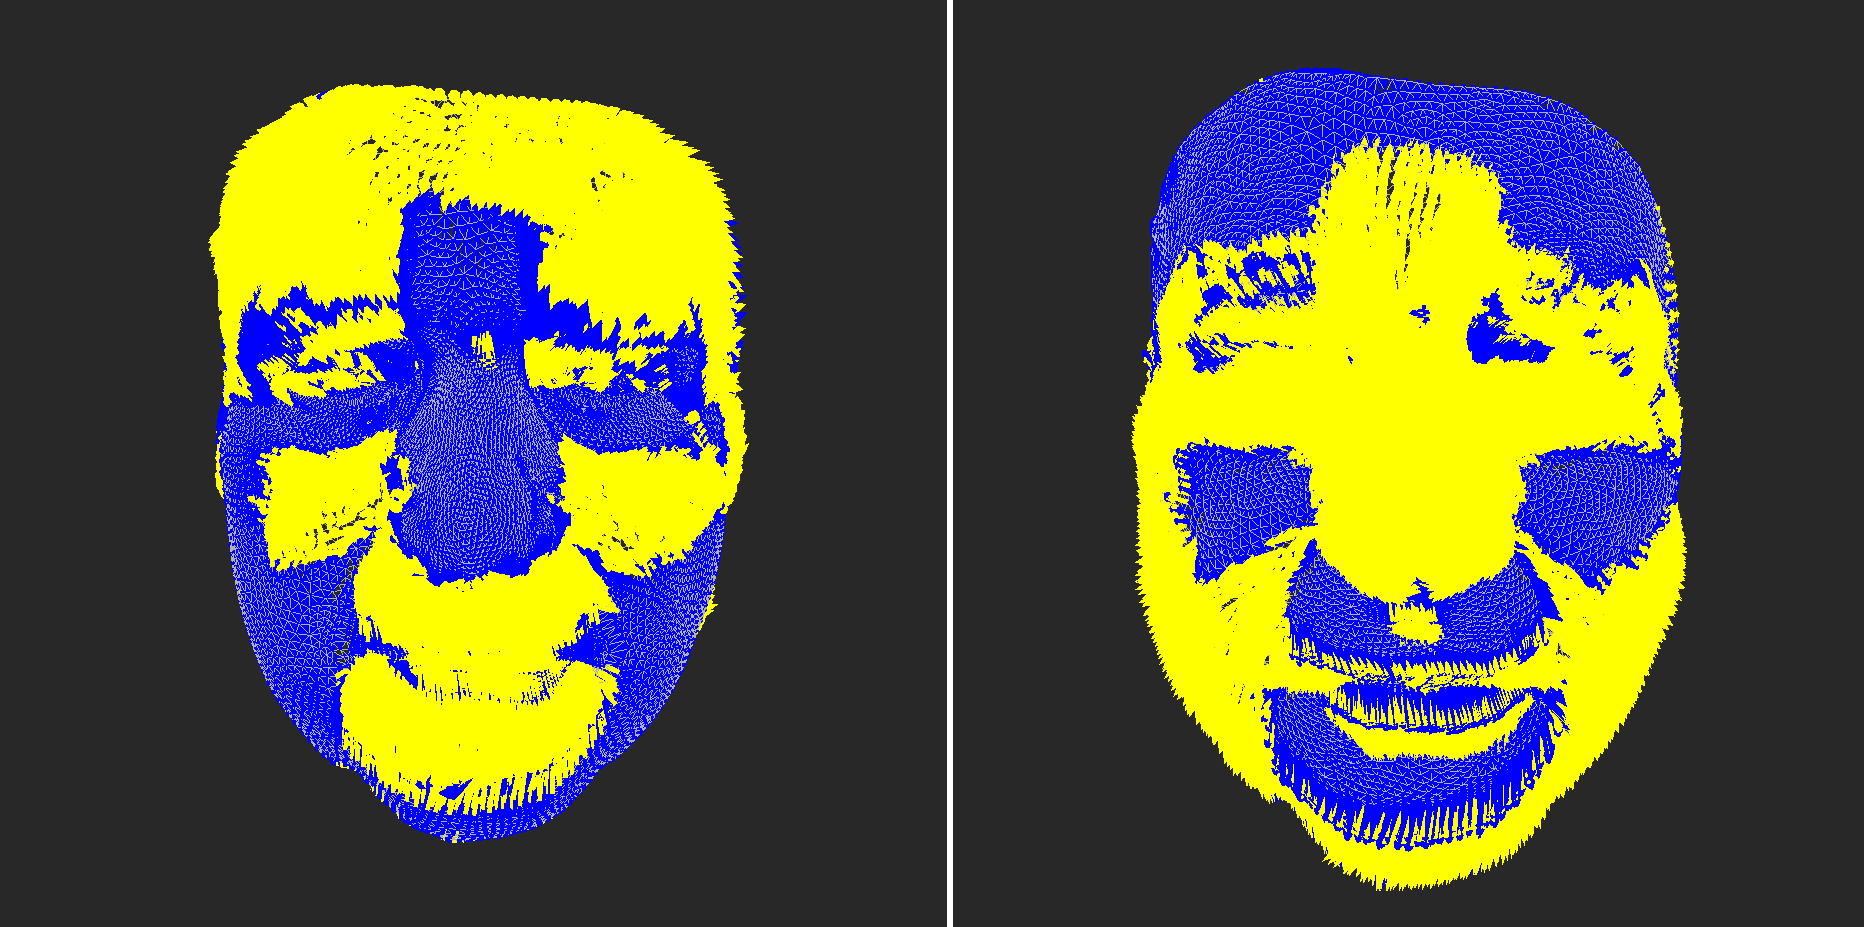
\includegraphics[width=\textwidth]{./img/meshdiff-unclustered_arrows.PNG}
\caption{MeshDiff - Vertex distance visualized by unclustered arrows}
\label{fig:meshdiff_unclustered}
\end{figure}
%%-----------------------------------------------------------------------------------------
%% SECTION
%%-----------------------------------------------------------------------------------------
\section{Vector Field Clustering}

As clustering is a very subjective task (see fig. \ref{fig:clustering_subjectivity}), each of the above mentioned papers has their own way of dealing with it.

\begin{figure}[h]
\centering
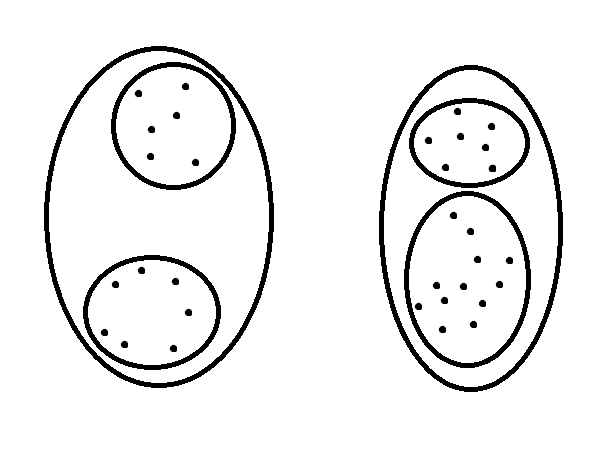
\includegraphics[width=0.6\textwidth]{./img/clustering_subjectivity.png}
\caption{The subjectivity of clustering - are there two or four clusters in the image?}
\label{fig:clustering_subjectivity}
\end{figure}

%%-----------------------------------------------------------------------------------------
\subsection{Overview of Vector Field Clustering Methods}

\citet{Telea99} use hierarchical (bottom-up) clustering where neighboring clusters with the smallest clustering error are merged. Each cluster has a representative vector and when merging, a weighted average of the two vectors is computed and assigned to the newly formed cluster. The paper introduced elliptic iso-error contours to compute the clustering error. The method is primarily aimed at 2D rectilinear vector fields but can be also used in 3D.

\citet{Garcke00} use a continuous clustering method based on the physical model of \citet{CahnHilliard58} which is used to describe phase separation and coarsening in binary alloys. This model is applied to vector field data which results in a diffusion problem rather than a splitting and merging problem. Such an algorithm also presumes an either 2D or 3D rectilinear grid.

\citet{Du04} use iterative (top-down) clustering where Voronoi regions are created around the initial cluster centers and a distance function is applied to each of them. The set of cluster centers which has the lowest value of the distance function is selected as the final cluster centers set. This method works with 2D and 3D rectilinear vector fields.

\citet{Peng12} use hierarchical clustering similar to \citet{Telea99}, only they use the GPU to compute the clustering by encoding a certain static view of a mesh into a rasterized image. The computation is then done for this specific image. To obtain the clustering error, a very simple formula is employed:

\begin{equation} \label{eq:clustering_error}
\bm{e}(C_1,C_2) = k_d \cdot \frac{d_{C_1C_2}}{d_{max}} + k_v \cdot \frac{v_{C_1C_2}}{v_{max}} + k_\alpha \cdot \frac{\alpha_{C_1C_2}}{\alpha_{max}} + k_m \cdot \frac{m_{C_1C_2}}{m_{max}}
\end{equation}

where \(k_d + k_v + k_\alpha + k_m = 1\). The other components are the following:

\begin{itemize}
\item \(d_{C_1C_2}\) is the Euclidean distance between the positions of the representative vectors of the clusters. The maximum distance \(d_{max}\) is the length of a diagonal of the geometry's bounding box
\item \(v_{C_1C_2}\) is the difference between the lengths of the representative vectors. The maximum velocity \(v_{max}\) is the largest length in the whole data set.
\item \(\alpha_{C_1C_2}\) is angle between the representative vectors. The maximum angle \(\alpha_{max} = 180^\circ\)
\item \(m_{C_1C_2}\) is the sum of the mesh resolutions of the two clusters. \(m_{max}\) is the largest value of \(m\) in the whole data set.
\end{itemize}

The mesh resolution component also differentiates this approach from all others because it represents an approximation of the density of the mesh in a given local area. Including it in the error formula assigns higher error to dense clusters which results in a larger amount of clusters (higher precision) in dense areas of the mesh and a smaller amount of clusters (lower precision) in sparse areas of the mesh. This method is therefore aimed at non-rectilinear 3D meshes.
%%-----------------------------------------------------------------------------------------
\subsection{Our Clustering Method}

For our clustering purposes, it is convenient to choose one of the presented methods and modify it if necessary. This approach saves time and gives us a baseline which we can improve upon. When selecting a clustering method, it is necessary to find a balance between simplicity and the ease of use (parameter tuning). We will lean towards simplicity in order to quickly obtain our baseline and only later look for improvements once we have a better idea of the actual performance of the selected method in our conditions.

While the hierarchical clustering of \citet{Telea99} is very simple and seems like a good candidate, its error function does not take into account the varying density of our triangle meshes and is also more demanding to use in 3D. In order to calculate the error function, one needs to find the elliptic iso-error contour of a given vector. This leads to cube-root equations which would have to be computed for every pair of clustering candidates. The error function of \citet{Peng12} (see eq. \ref{eq:clustering_error}), on the other hand, is both sensitive to non-uniform meshes and computationally simpler and more scalable into higher dimensions.

Lastly, we will not use the GPU-based clustering computation from \citet{Peng12} because we need to be able to view the resulting visualizations easily from various angles in real time. The basic approach in \citet{Telea99} computes the clustering once for the whole vector field.

Our clustering method will use the hierarchical algorithm from \citet{Telea99} and the error function \ref{eq:clustering_error} from \citet{Peng12}. Merging of two clusters will be done by computing a weighted average of their representative vectors.
%%-----------------------------------------------------------------------------------------
\subsection{Algorithm}

Here is the pseudocode of the hierarchical clustering algorithm as presented in \citet{Telea99}:

\begin{algorithm}[H]
\caption{Clustering}
\begin{algorithmic}[1]

\Require ClusterSet s
\Statex
\For{all cells cell\textsubscript{i} \textbf{in} dataset}
	\State c = makeCluster(cell\textsubscript{i});
    \State set level of c to 0;
    \State add c to s;
\EndFor
\Statex
\For{all clusters c\textsubscript{i} in s}
	\For{all clusters c\textsubscript{j} neighbours of c\textsubscript{i}}
    	\State e = clusteringError(c\textsubscript{i}, c\textsubscript{j});
        \State insert pair (c\textsubscript{i}, c\textsubscript{j}) in increasing order of error e in a hash table;
        \State mark c\textsubscript{i} and c\textsubscript{j} as NOT\_CLUSTERED;
    \EndFor
\EndFor
\Statex
\State int i = 0;
\For{all pairs (c\textsubscript{i}, c\textsubscript{j}) in increasing order of error in the hash table}
	\If{both c\textsubscript{i} and c\textsubscript{j} are NOT\_CLUSTERED}
    	\State c = mergeClusters(c\textsubscript{i}, c\textsubscript{j});
        set level of c to l++;
        mark c\textsubscript{i} and c\textsubscript{j} as CLUSTERED;
        \For{all neighbors n\textsubscript{i} of c}
        	\State e = clusteringError(c, n\textsubscript{i});
            insert pair (c, n\textsubscript{i}) in order in hash table
        \EndFor
    \EndIf
\EndFor
\Statex
\Return c as root of tree
\end{algorithmic}
\end{algorithm}

There are two important functions in the algorithm, \texttt{clusteringError()} and \texttt{mergeClusters()}. \texttt{clusteringError()} uses formula \ref{eq:clustering_error} to compute the clustering error and therefore directly influence which clustering candidates will be merged first. \texttt{mergeClusters()} constructs the representative vector of the new cluster by computing a weighted average of the representative vectors of the merged clusters where the weight is the geometrical area of the clusters.
%%-----------------------------------------------------------------------------------------
\subsection{Improvements}

We also made one modification of the clustering algorithm which can be optionally turned on in the experimental application MeshDiff.

When we consider the surface of a triangle mesh with our vector field placed in the vertices of the mesh, there are two types of vectors - those pointing "inside" the mesh and those pointing "out" of the mesh. We found out that it might be useful to add one more condition to the clustering process and only allow those clusters to be merged whose representative arrows point in the same direction as outlined above. We say that such vectors have the same orientation.

The result of such a clustering is then a forest instead of a tree. This may result in certain clusterings not covering the whole mesh which does not necessarily lower the quality of the resulting visualization but should nevertheless be taken into account.
%%-----------------------------------------------------------------------------------------
%% SECTION
%%-----------------------------------------------------------------------------------------
\section{Proposed Visualizations}

(focus on the visual appearance)

\begin{itemize}
\item what kind of metrics are used
\item how is the clustering connected to this
\item what does it look like and how can the user set it
\item what is it assumed to be good for 
\end{itemize}

\subsection{Cluster Color}

\subsection{Arrows}

\subsection{Thresholding}
